\documentclass{article}
\usepackage{neurips_data_2024}
\usepackage[utf8]{inputenc} % allow utf-8 input
\usepackage[T1]{fontenc}    % use 8-bit T1 fonts
\usepackage{hyperref}       % hyperlinks
\usepackage{url}            % simple URL typesetting
\usepackage{booktabs}       % professional-quality tables
\usepackage{amsfonts}       % blackboard math symbols
\usepackage{nicefrac}       % compact symbols for 1/2, etc.
\usepackage{microtype}      % microtypography
\usepackage{xcolor}         % colors
\usepackage{lipsum}
\usepackage{graphicx}       % include pdfs as figures
\usepackage[ruled]{algorithm2e}
\usepackage{bm}

\title{\texttt{metabench}\\A Sparse Benchmark to Measure General Ability\\in Large Language Models}
\author{%
   Alex Kipnis $^{1}$ \thanks{Correspondence to \texttt{adkipnis@mailbox.org}} \quad
   Luca M. Schulze Buschoff $^{1}$ \quad
   Konstantinos Voudouris $^{1,2}$ \quad
   Eric Schulz $^1$\\
   $^1$ Human-Centered AI, Helmholtz Munich \quad $^2$ University of Cambridge\\
}

\begin{document}

\maketitle

\begin{abstract}
   Large Language Models (LLMs) vary in their abilities on a range of tasks. Initiatives such as the \texttt{Open LLM Leaderboard} aim to quantify these differences with several large benchmarks (sets of test items to which an LLM can respond either correctly or incorrectly).
   However, high correlations within and between benchmark scores suggest that (1) there exists a small set of common underlying abilities that these benchmarks measure, and (2) the latter tap into redundant information and may thus be considerably compressed.
   We use data from over $5.000$ LLMs to analyze the psychometric properties of six benchmarks (\texttt{ARC}, \texttt{GSM8K}, \texttt{HellaSwag}, \texttt{MMLU}, \texttt{TruthfulQA} and \texttt{WinoGrande}) in order to identify their most informative items.
   Using this subset, we construct a sparse benchmark, \texttt{metabench}, that has less than $4$\% of the original size of all six benchmarks combined. Moreover, \texttt{metabench} goes beyond point scores by yielding estimators of the underlying benchmark-specific abilities.
   We show that these estimators (1) can be used to reconstruct the original \textit{individual} benchmark scores, and (2) have one underlying common factor which can be used to reconstruct the original \textit{total} score with $\sim 2$\% error.
\end{abstract}

% ------------------------------------------------------------------------------------
% Introduction
\section{Benchmarks do not need to be big}
\subsection{Related Work}
% ------------------------------------------------------------------------------------
% Methods
\section{Benchmark Distillation}
\begin{figure}[h]
   \centering
   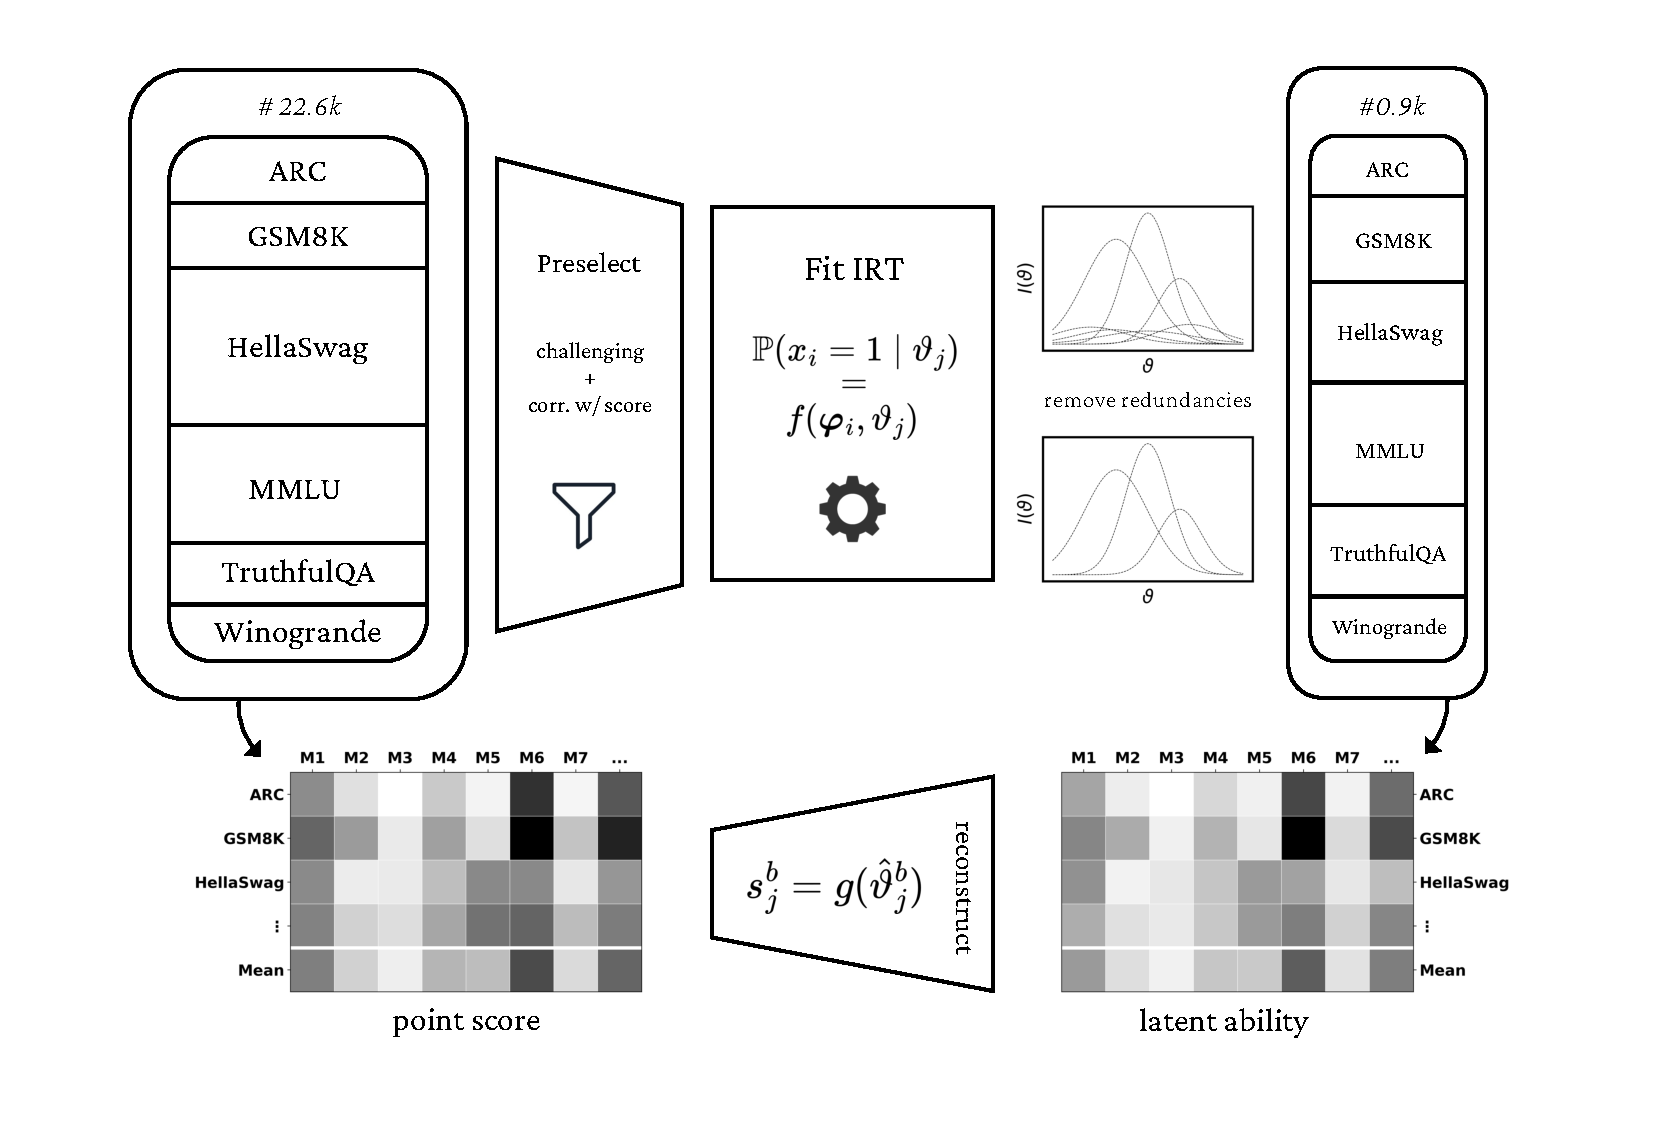
\includegraphics[width=0.9\textwidth]{figures/overview.pdf}
   \caption{\textit{Processing pipeline}. (1) Collect item-wise accuracies from all available LLMs for each benchmark on \texttt{Open LLM Leaderboard}. (2) Remove items solved by more than $95\%$ of LLMs and items with part-whole correlation $r \approx 0$. (3) Fit variants of IRT models to the remaining items and choose the best fit by cross-validation. (4) Infer item information from the item parameters and filter out uninformative items to (5) construct \texttt{metabench}. (6) Use the item parameters to estimate the benchmark-specific abilities and use factor analysis to find a common factor. (7) These can be used to reconstruct the original (normalized) benchmark scores as well as their mean.}
   \label{fig:overview}
\end{figure}

\subsection{Data Collection and Preprocessing}
% openllm leaderboard
We collected openly available item-wise accuracies from \href{https://huggingface.co/datasets}{Hugging Face Datasets} for the six benchmarks that are part of the \href{https://huggingface.co/open-llm-leaderboard}{\texttt{Open LLM Leaderboard}}: \texttt{ARC}, \texttt{GSM8K}, \texttt{HellaSwag}, \texttt{MMLU}, \texttt{TruthfulQA} and \texttt{WinoGrande}. % TODO: add citation
After excluding flagged and merged models, we obtained data from $1355$ unique users, yielding in total $6875$ LLMs out of which $5055$ had data for all six benchmarks. 
For comparability, we normalized the benchmark scores on a percent scale and saved for future reference. Per benchmark, we removed LLMs with the lowest $0.1\%$ of scores to reduce noise.
Items with duplicate prompts, standard deviation below $1\%$ and easiness above $95\%$ were removed. We then estimated the part-whole correlation between  items and the total score using the point-biserial correlation coefficient:
\begin{equation}
   r_{pbis} = \frac{\mu_1 - \mu}{s_{n-1}} * \sqrt{\frac{n_1 * (n-n_1)}{n*(n-1)}},
\end{equation}
where $\mu_1$ resp. $\mu$ are the mean scores of the group who answered the item correctly resp. the total group, $s_{n-1}$ is the standard deviation of the total group, $n_1$ resp. $n$ are the size of the group that answered the item correctly resp. the total group. Items with $r_{pbis} = 0 \pm \epsilon$ were removed, $\epsilon$ was set to $0.05$ except for \texttt{Winogrande} where it was set to $0.02$ as otherwise hundreds of items would have been removed.\footnote{Note that it is customary to remove items with negative $r_{pbis}$. However, items with a negative $r_{pbis}$ \textit{do} contain information about the benchmark score. We therefore chose to keep them.}
For comparability, we conducted a train-test-validation split of the LLMs in the following manner: For stratification, we calculated the grand average (GA) of the original benchmark scores for models that had data for \textit{all six} benchmarks, and used it to split off $10\%$ of the LLMs as the global test set. For cross-validation per benchmark, we split off further $10\%$ of the remaining LLMs as the local validation set, this time stratifying by the specific benchmark score. 

\subsection{Evolutionary Subsampling}
After preprocessing, \texttt{HellaSwag} and \texttt{MMLU} still had substantially more items than LLMs, prohibiting the use of IRT models. To further reduce their number of items to $1/4$ of the respectively available LLMs, we used an evolutionary subsampling approach:
\begin{enumerate}
   \item Randomly drop $k$ items from the benchmark.
   \item Re-calculate the mean score $\dot {\boldsymbol{\mu}}$ of the remaining items for each LLM.
   \item Fit a non-linear regression model on the training set: $\boldsymbol\mu = f(\dot{\boldsymbol\mu})$ 
   \item Calculate the root mean square error (RMSE) on the validation subset.
\end{enumerate}
This inner loop is repeated $50$ times, and the iteration with the lowest RMSE makes the cut. The outer loop is repeated until the number of items reaches the goal size. The final set of items and and the final regression model are tested on the global test set. For \texttt{MMLU}, the procedure uses a linear model of all scenario scores to predict the total score, but is otherwise identical.
Using this procedure, we reduced the number of items in \texttt{HellaSwag} from $10042$ to $1181$ and in \texttt{MMLU} from $14042$ to $1108$ with minimal loss in predictive performance.
\begin{figure}[h]
   \centering
   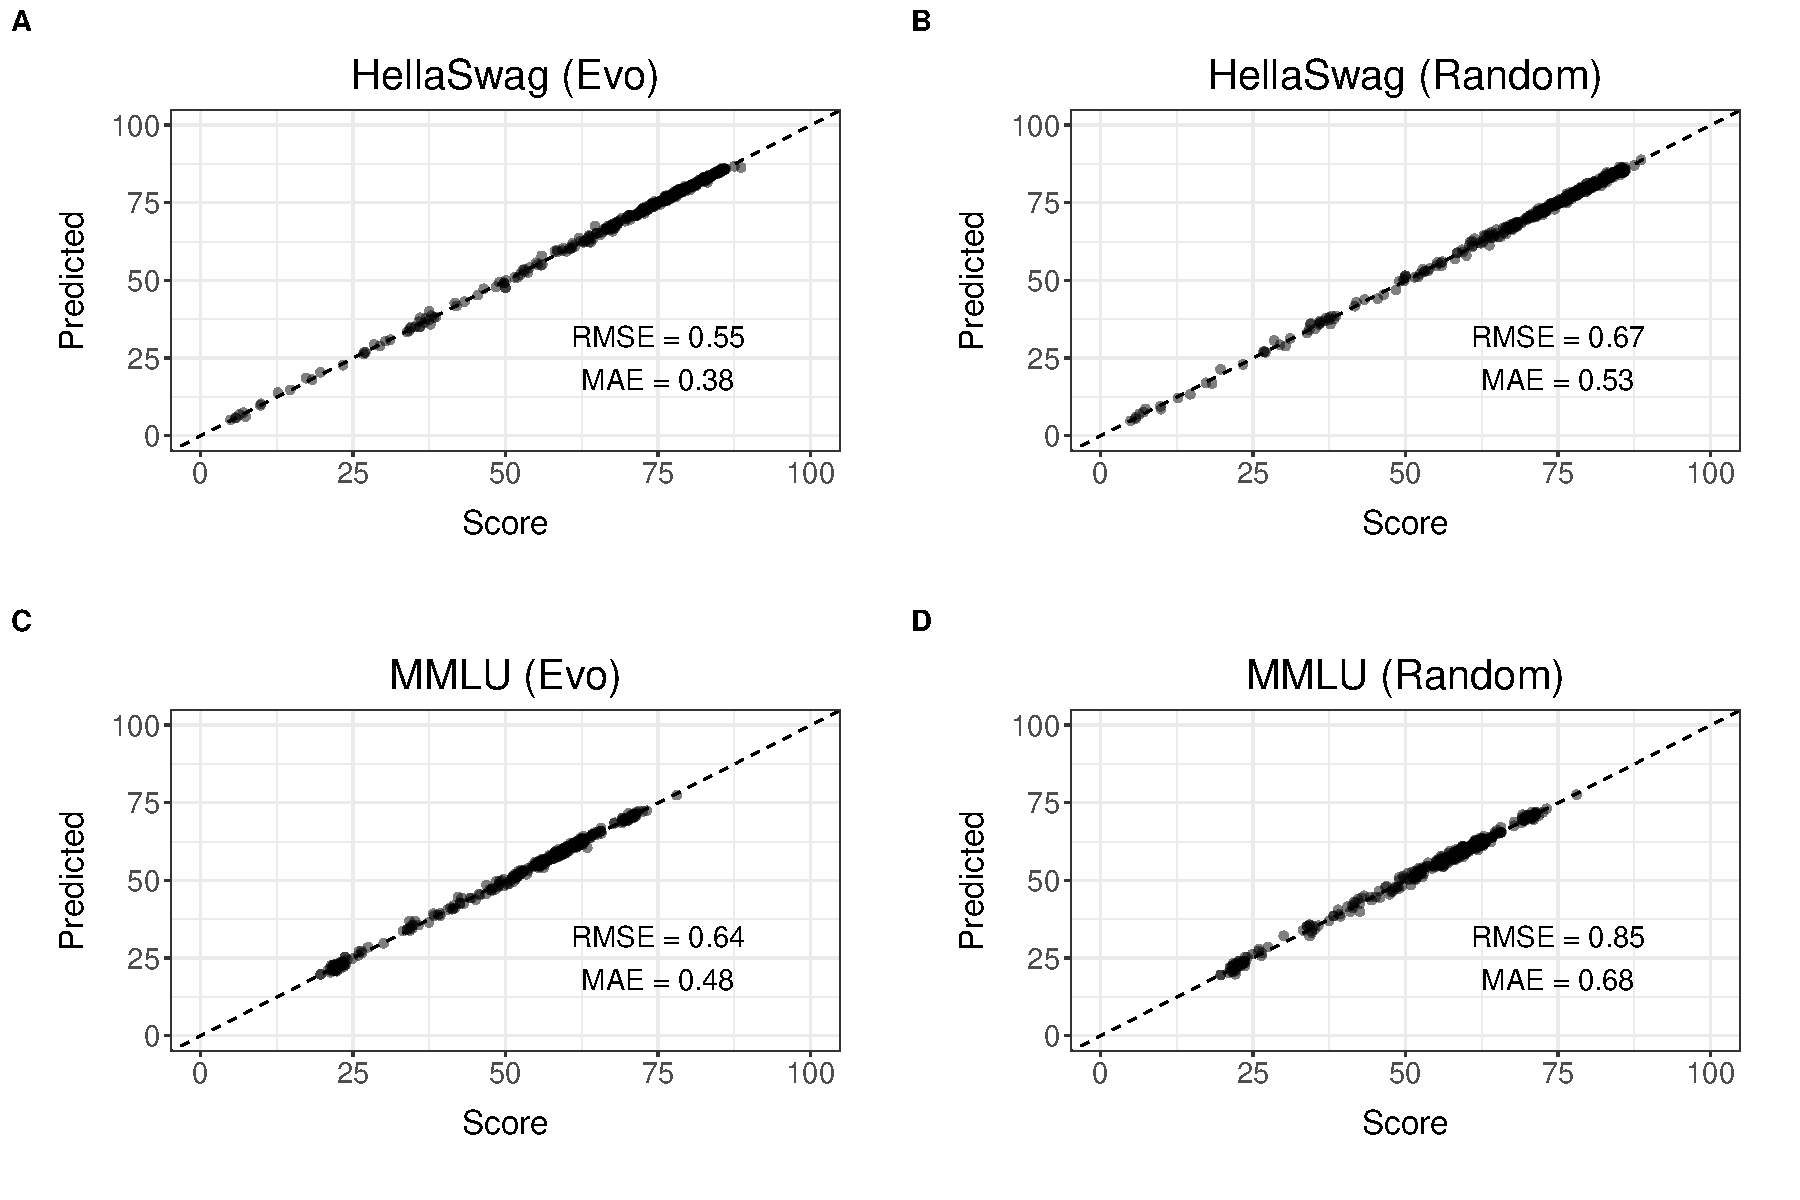
\includegraphics[width=0.8\textwidth]{figures/evo.pdf}
   \caption{\textit{Score reconstruction after evolutionary subsampling}. Normalized mean scores reconstructed for the test set using items selected by the evolutionary subsampling procedure (A,C) vs. a random selection of the same size (B,D).}
   \label{fig:hs-reduced}
\end{figure}

\subsection{Item Response Theory}
% IRT in a nutshell
Item response theory (IRT) is a branch of psychometrics that models the relationship between a person's ability and the probability of a correct response to an item. It is closely related to factor analysis, but assumes binary or polytomous responses. %TODO cite
Let $x_{ij}$ be the accuracy of item $i$ for subject $j$ with some (unknown) latent ability $\boldsymbol \vartheta_j$, then the probability of a correct response is modeled as:
\begin{equation}
   \mathbb P(x_{ij}=1|\boldsymbol \vartheta_j) = f(x_{ij}|\boldsymbol \vartheta_j, \boldsymbol \alpha_i),
\end{equation}
where $f$ is a link function and $\boldsymbol \alpha_i$ are the item parameters. A simple IRT model is the 2-parameter logistic model (2PL) with $\boldsymbol \alpha_i = (d_i, \mathbf a_i)$ and $f(x_{ij}|\boldsymbol \vartheta_j, \boldsymbol \alpha_i) = G(\mathbf a_i^\top  \boldsymbol \vartheta_j - d_i)$, where $G$ is the logistic function, $\mathbf a_i$ is the loading parameter and $d_i$ is the difficulty parameter.\footnote{Generally, $\mathbf a_i$ can be a vector, but parameter recovery scales poorly with the dimensionality of this vector. As higherdimensional IRT models require much larger subjects-to-items ratios than in our case, we chose to only estimate unidimensional models.} The primary goal is to estimate the item parameters $\mathbf A = (\boldsymbol \alpha_i)_{i = 1, \ldots, d}$. As the latent ability is generally also unkown, the gold-standard approach is to use marginal maximum likelihood methods, which treat the latent ability as a random variable and attempt to maximize $\mathcal L(\mathbf A) = \prod_{i=1}^n \int \prod_{j=1}^d f(x_{ij}|\boldsymbol \vartheta_i, \boldsymbol\alpha_j) f(\boldsymbol \vartheta_i) \, \mathrm d\boldsymbol \vartheta_i$. Due to the integral there is no analytical solution to this problem, but it can be approximated using Expectation-Maximization (EM) algorithms. %TODO cite
After model fitting, $\boldsymbol \vartheta_j$ can be estimated for each subject $j$ using e.g. maximum a posteriori estimation. %TODO cite

% what we do
We use the \texttt{mirt} package in R to fit a range of IRT models to the remaining items, using EM with semiparametric density estimation of the latent ability, as the normality assumption We compare the empirical distributions of GA scores for (1) all LLMs vs. (2) all latest LLMs per user to gauge how severely the conditional independence assumption of IRT models is violated. As the distributions are nearly identical and as the ratio between LLMs and items is already low for IRT standards, we treat all LLMs as independent observations.

%
% We fit a range of IRT models to the remaining items using the \texttt{mirt} package in R. We used the Expectation-Maximization algorithm with semiparametric density estimation of the latent ability $\boldsymbol \vartheta$. 
% There were multiple LLMs per user, which could pose a problem for the conditinal independence assumption of IRT models. To gauge how severely this assumption was violated, we compared the empirical distributions of GA scores for (1) all LLMs vs. (2) all latest LLMs per user. As the distributions were nearly identical and as the ratio between LLMs and items was already low for IRT standards, we decided to treat all LLMs as independent observations.
%
% estimate theta posterior per model
% fit gam to recover full score
% test on validation set
\subsection{Information Filtering}
% item characteristic curves
% item information
% information sweep and bayesian hyperparameter optimization

% ------------------------------------------------------------------------------------
%  Results
\section{Score Reconstruction}
% reconstruction of individual scores
% reconstruction of total score
% exploratory factor analysis

% ------------------------------------------------------------------------------------
%  Discussion / Conclusion
\section{Going Beyond Point Scores}
\section{Conclusion}
\subsection{Limitations}
\subsection{Future Work}

% ------------------------------------------------------------------------------------
%  Appendix
\section*{Acknowledgments}
\section*{References}
\section*{Appendix}
\end{document}
